% Restructured book: system construction from the non-evaluation parts of old Chapter 4.
\chapter{System Construction}

This chapter presents the construction of RoomFlow as a complete web-based interior design system. This chapter explains how these components are integrated into an interactive application. The focus is on the system architecture, frontend workspace, backend processing pipeline, database design, implemented functions, and deployment environment. The chapter first introduces the overall architecture and package organization, then describes the detailed design of the user interface, backend services, rendering flow, and data model. It also presents the main implemented functions of RoomFlow, including room editing, automatic layout generation, 3D preview, photorealistic rendering, image editing, and result management.

\section{Architecture Design}\label{sec:architecture-design}

The system follows a client-server architecture. The frontend is a React single-page application responsible for user input, 2D floor-plan editing, layout comparison, 3D preview, render control, account screens, and saved-design interactions. The backend is a FastAPI service responsible for authentication, inventory access, layout generation, artifact retrieval, image rendering, saved layouts, and generated-render storage. PostgreSQL stores user data, inventory metadata, saved layout cases, saved layouts, authentication sessions, and render records. External AI services are used for LLM-based semantic planning and for image generation or editing. When retrieval or semantic matching is needed, embedding services can support inventory or knowledge lookup. Provider keys and model configuration are handled only by the backend. In the implementation reported in this thesis, the backend provider configuration uses \texttt{gpt-5.4-mini} for text-based planning and visual preflight tasks, and \texttt{gpt-image-2} for photorealistic image generation and localized image editing.

\subsection{Software Architecture Selection}\label{subsec:software-architecture-selection}

A separated frontend-backend architecture was selected because the application combines intensive user interaction with long-running AI workflows. The browser is the right place for drawing, dragging, camera control, and immediate preview. The backend is the right place for API keys, database access, case persistence, model configuration, and controlled execution of LLM and solver modules. This separation also improves deployment because the API can be protected and scaled independently from the static frontend.

A client-only web application was not selected because it would expose provider keys and make persistent artifact storage difficult. A monolithic desktop application would also make the shared backend pipeline, account data, and reproducible experiment artifacts harder to manage. The web client-server design keeps the interaction lightweight while still allowing the backend to manage authentication, database writes, reproducible pipeline artifacts, and provider calls.

\subsection{Overall Design}\label{subsec:overall-design}

The overall design follows a pipeline data flow. The user enters the room, style, and design requirements in the frontend. The frontend sends the prepared floor-plan geometry, openings, room type, and brief to the backend. The backend creates a case folder, records metadata and stage status, runs the layout pipeline, and returns final layout variants. The frontend converts the selected variant into the common DesignPlanV1 structure, displays it in 2D and 3D, and optionally sends a 3D snapshot to the image-rendering workflow.

Every pipeline run writes reproducible artifacts under a case folder. These artifacts include module outputs, normalized inputs, status files, layout variants, and evaluation artifacts. This design is useful for debugging because a failed run can be inspected at the stage where it failed instead of being treated as a single opaque model response.

Figure~\ref{fig:6-1} summarizes the overall architecture and the high-level data flow among browser, backend services, AI services, storage, and evaluation runners.

\begin{figure}[!htbp]
\centering
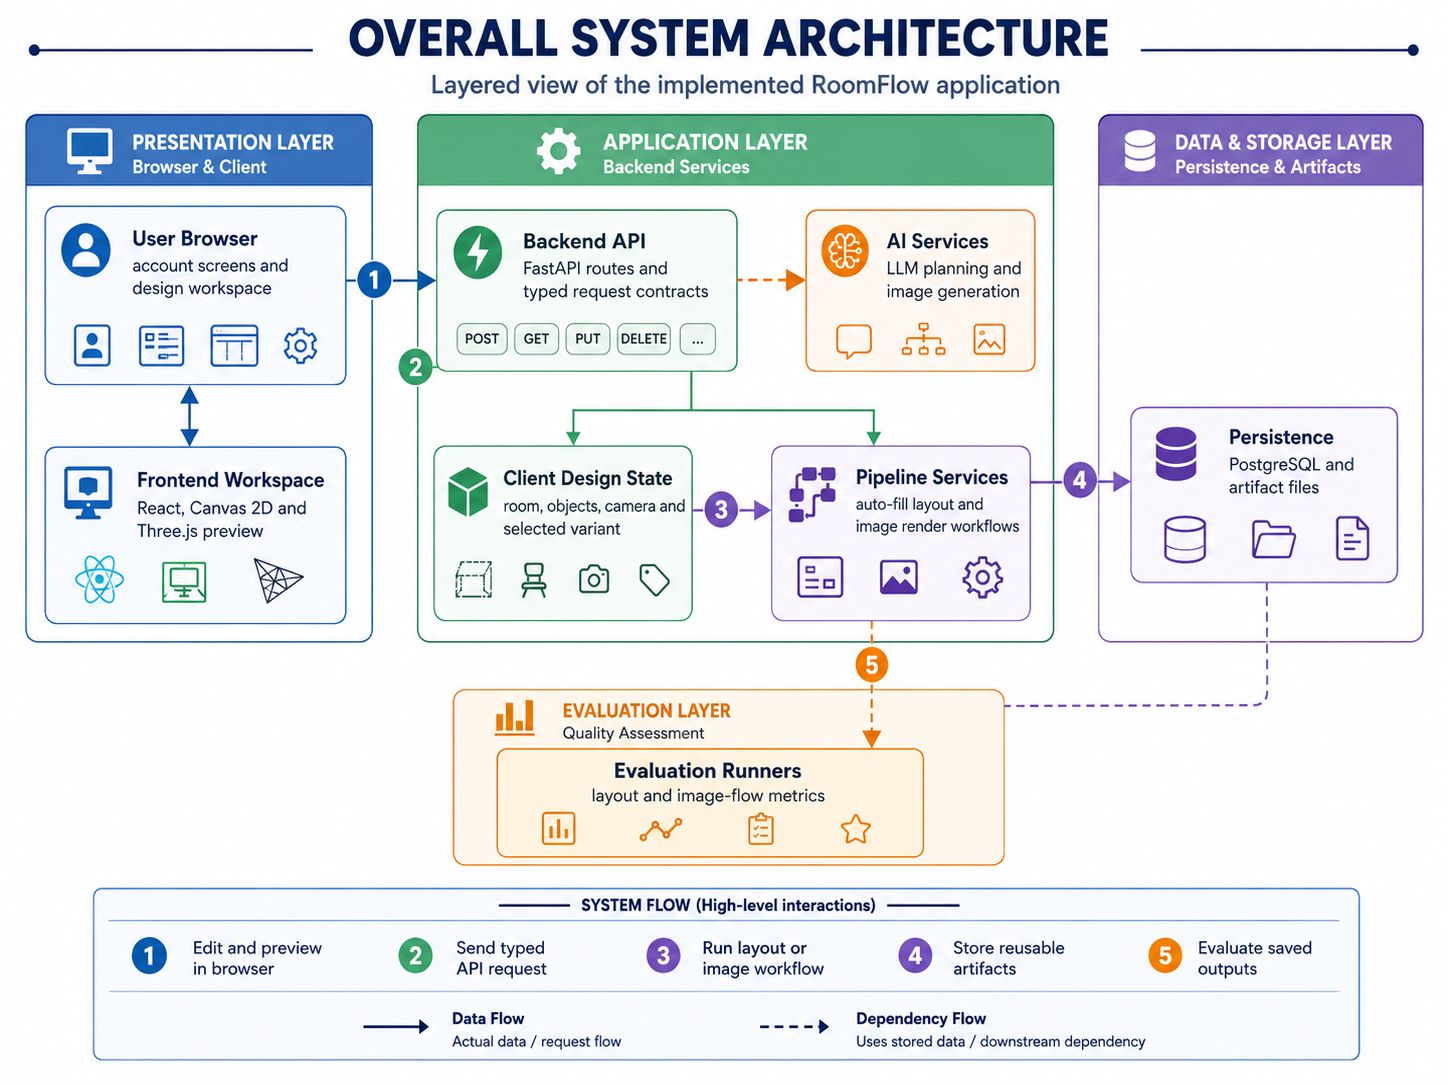
\includegraphics[width=\textwidth]{figures/chapter4/figure_01.png}
\caption{Overall system architecture of RoomFlow.}
\label{fig:6-1}
\end{figure}

The numbered arrows in Figure~\ref{fig:6-1} summarize the runtime flow: the user edits design state in the frontend, the backend executes the layout or image pipeline, persistence stores the resulting layouts and renders, and evaluation runners reuse saved artifacts without becoming part of the interactive user path. The frontend owns direct manipulation and visualization; the backend owns AI calls, geometry validation, persistence, and reproducible artifacts.

\subsection{Package Design}\label{subsec:package-design}

The backend package design follows a layered responsibility split. API packages expose routes and request handlers. Application-service packages orchestrate layout generation, image rendering, saved layouts, and inventory operations. Domain packages contain the LLM-facing planning modules, object-program construction, geometric solver, style binding, and gallery selection. Infrastructure packages provide database access, artifact storage, configuration, and external provider clients. Evaluation and experiment packages are kept separate from runtime routes so that benchmark scripts can reuse the same core modules without changing the API layer.

This organization keeps pure planning and solving logic separate from HTTP and database concerns. It also makes ablation testing practical because individual modules can be disabled or replaced without changing the entire API surface.

Figure~\ref{fig:6-2} shows the package dependency direction used to preserve this separation between routes, services, domain modules, infrastructure, and evaluation utilities.

\begin{figure}[!htbp]
\centering
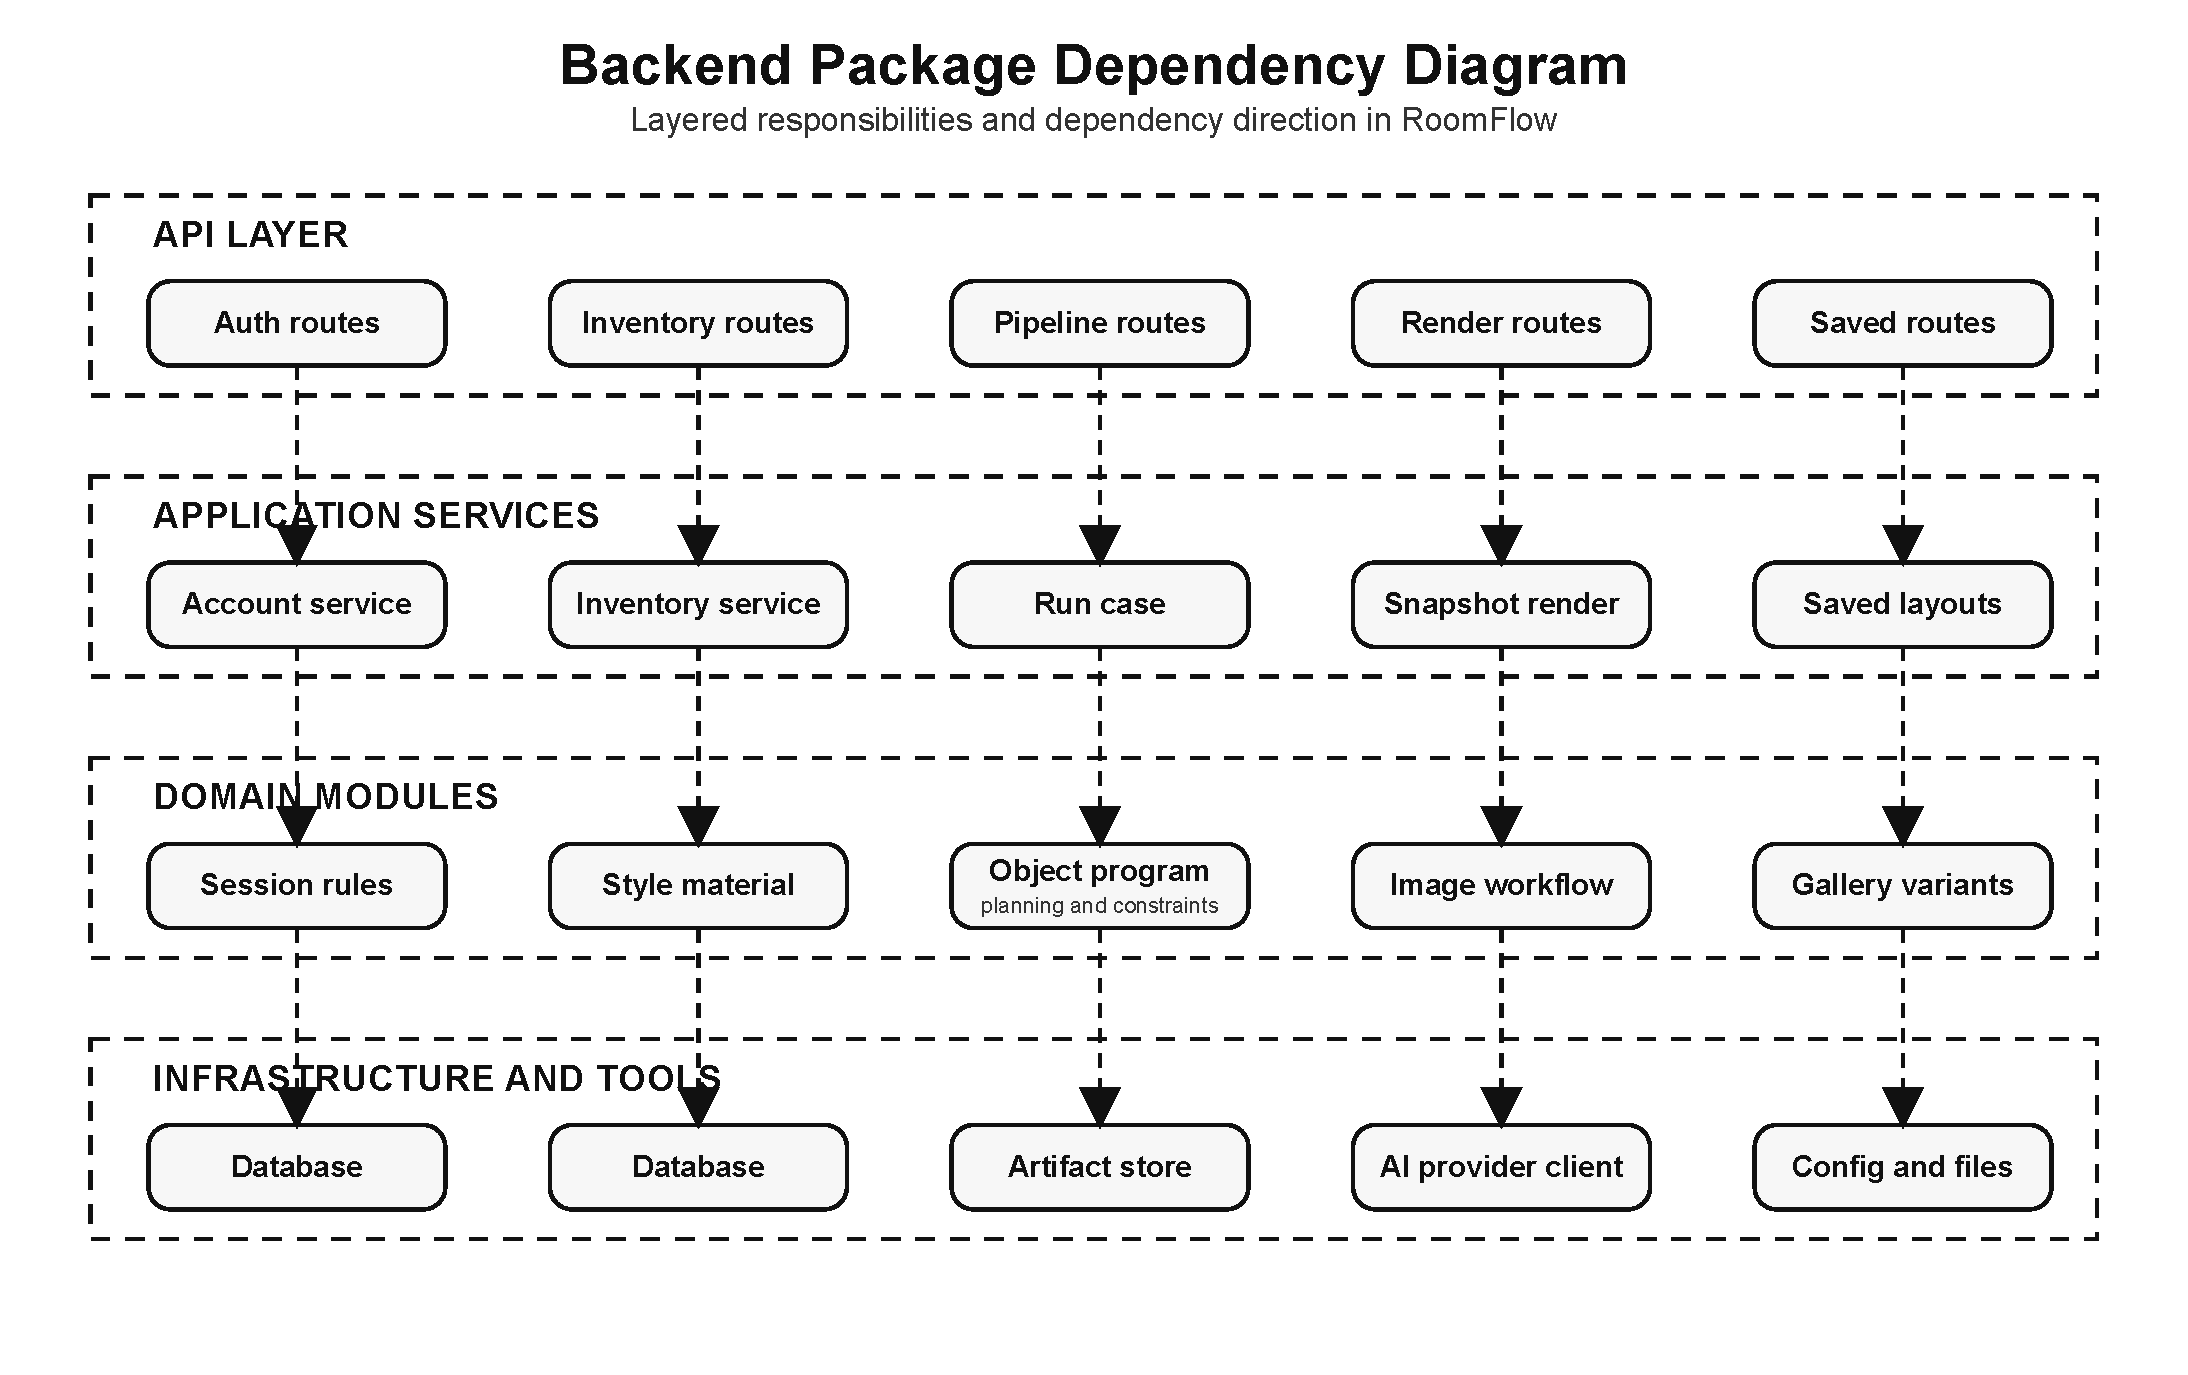
\includegraphics[width=\textwidth]{figures/chapter4/figure_02.pdf}
\caption{Backend package dependency diagram.}
\label{fig:6-2}
\end{figure}

Figure~\ref{fig:6-2} also shows that API routes depend on services and pipeline orchestration, while pipeline code depends on domain planning, solving, styling, and image-flow modules. Persistence, configuration, and external clients stay at the infrastructure boundary.

\section{Detailed Design}\label{sec:detailed-design}

\subsection{User Interface Design}\label{subsec:user-interface-design}

The user interface is organized around a single design workspace. The input panel collects the room type, style, design brief, and other design parameters. The 2D canvas displays the room boundary, walls, openings, and furniture footprints, and supports direct manipulation such as moving, rotating, replacing, or deleting objects. The layout-variant panel allows the user to compare automatically generated options. The 3D preview panel reconstructs the selected layout and provides camera and rendering controls. Account and saved-artifact screens handle sign-in, saved layouts, render history, and inventory-related functions.

The UI uses direct manipulation. A user can select a wall, door, window, or furniture item and update it without editing raw JSON. Internally, the application keeps geometry in millimeters and converts it to pixels only for drawing. This prevents visual edits from corrupting the backend representation and keeps 2D, 3D, and evaluation outputs aligned.

\subsection{Backend Pipeline Design}\label{subsec:backend-pipeline-design}

The backend auto-fill flow is implemented as a sequence of stages controlled by the pipeline orchestrator. The first stage prepares the case: it loads manual placements, creates a case id, writes metadata, and normalizes the room input. The second stage performs semantic planning: it interprets the room, compiles style preferences, generates object clusters, extracts request priorities, and decides object counts. The third stage converts the semantic output into a solver-ready object program with anchors, relations, and constraints. The fourth stage runs the geometric solver to search for absolute object placements using the room boundary, openings, furniture footprints, manual constraints, and relation plans. The final stage selects gallery-eligible variants, attaches inventory and style metadata, writes artifacts, and returns the selectable payload to the frontend.

If the final candidates are too similar, the pipeline attempts to create additional valid variants by changing high-level anchor choices, such as the wall used by the bed or sofa, the main media-wall direction, or the circulation pattern. This diversification step is used only after the solver has found valid layouts. Its purpose is not to repair one invalid layout locally, but to make the gallery contain meaningfully different options for user comparison.

Figure~\ref{fig:6-3} traces this backend flow from the frontend request through planning, solving, persistence, and the returned gallery payload.

\begin{figure}[!htbp]
\centering
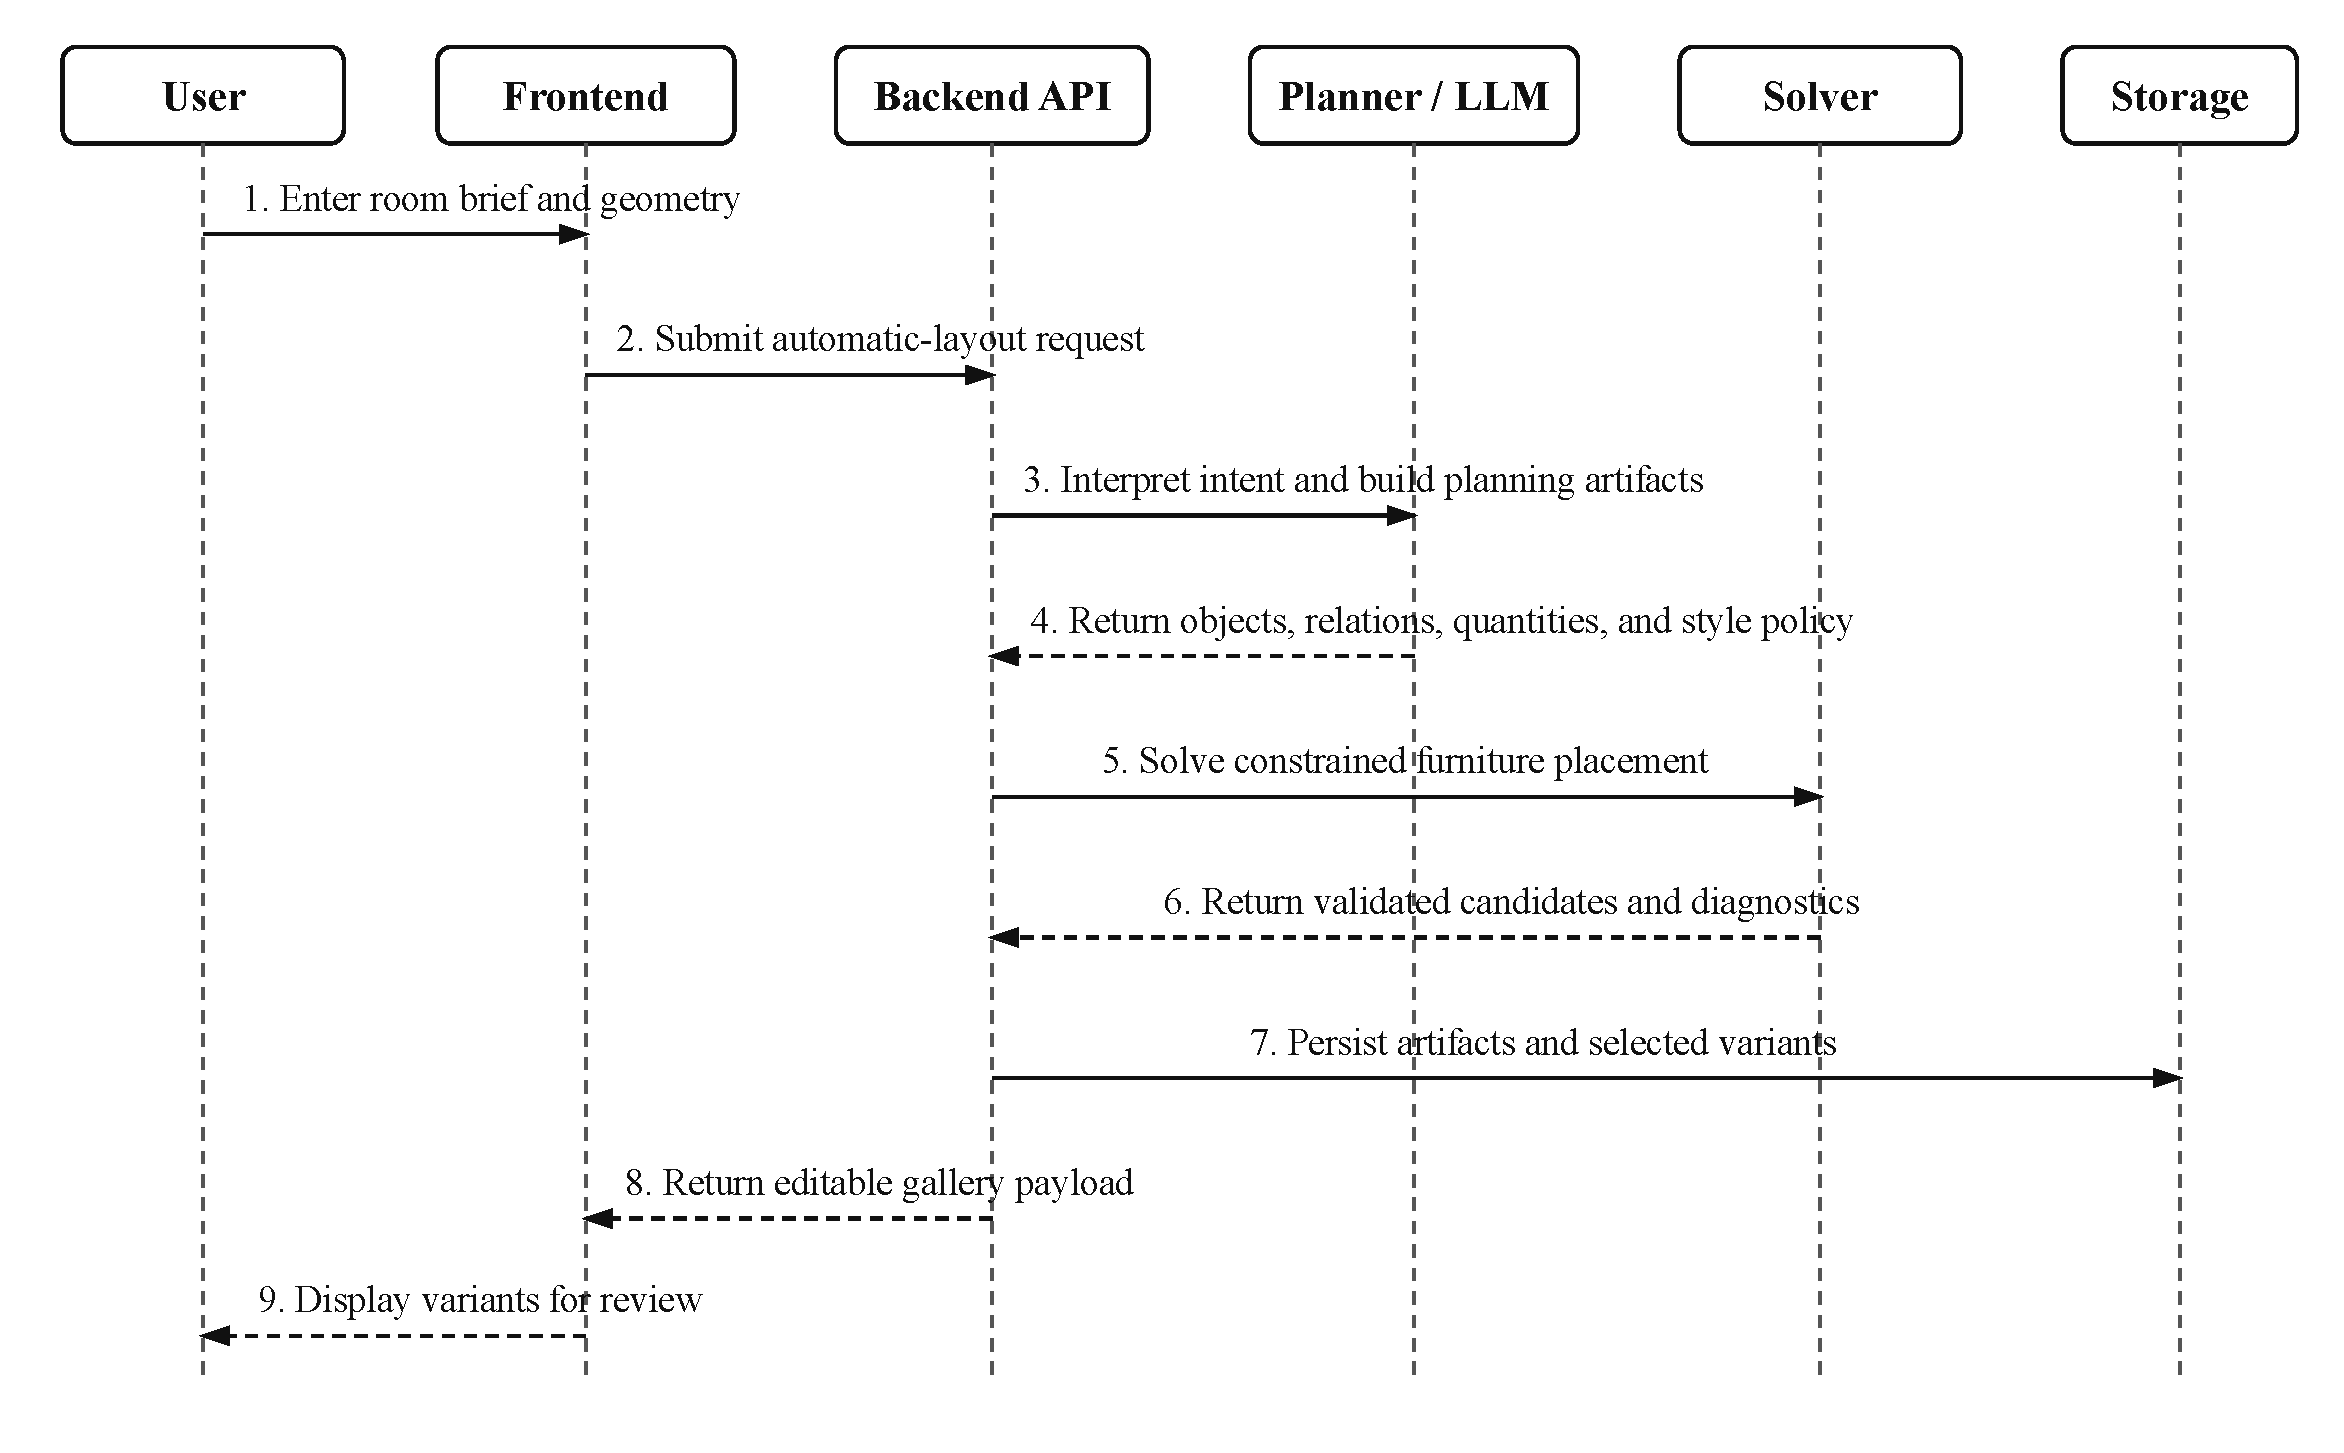
\includegraphics[width=\textwidth]{figures/chapter4/figure_03.pdf}
\caption{Sequence diagram of the auto-fill furniture layout flow.}
\label{fig:6-3}
\end{figure}

Figure~\ref{fig:6-3} shows why the auto-fill workflow is auditable. Each major step returns structured artifacts before the solver and final gallery selector produce the user-facing layout variants.

The implemented flow is asynchronous from the user's perspective. The backend writes stage status and streams progress events so the frontend can show that the room interpretation, planning, solving, and gallery selection stages are running. If a provider call fails, the backend records the failed stage and returns a recoverable error. If the solver cannot find a valid layout, the response contains diagnostics instead of an empty success payload.

\subsection{3D Snapshot and Image Rendering Design}\label{subsec:3d-snapshot-and-image-rendering-design}

The image rendering module uses the selected 3D layout as the source of truth. The frontend captures a snapshot payload containing the source 3D snapshot, visible objects, screen-space bounding boxes, room shell facts, opening facts, camera metadata, and optional references. The backend snapshot prompt compiler converts this payload into a structured prompt with object facts, spatial relations, occlusion information, and strict layout constraints.

The renderer supports three user-facing modes: generating a new render from a selected 3D snapshot, editing an existing render with a localized request, and re-rendering from a different camera view. The evaluation code can additionally run ablation variants of the generation workflow, such as text-only prompting, text contracts, visual preflight, and locked-geometry references. These variants are used for Chapter 8 experiments, while the user-facing workflow exposes only the selected generation and editing controls.

Figure~\ref{fig:6-4} shows the sequence used when a selected 3D snapshot is converted into a provider request and saved render artifact.

\begin{figure}[!htbp]
\centering
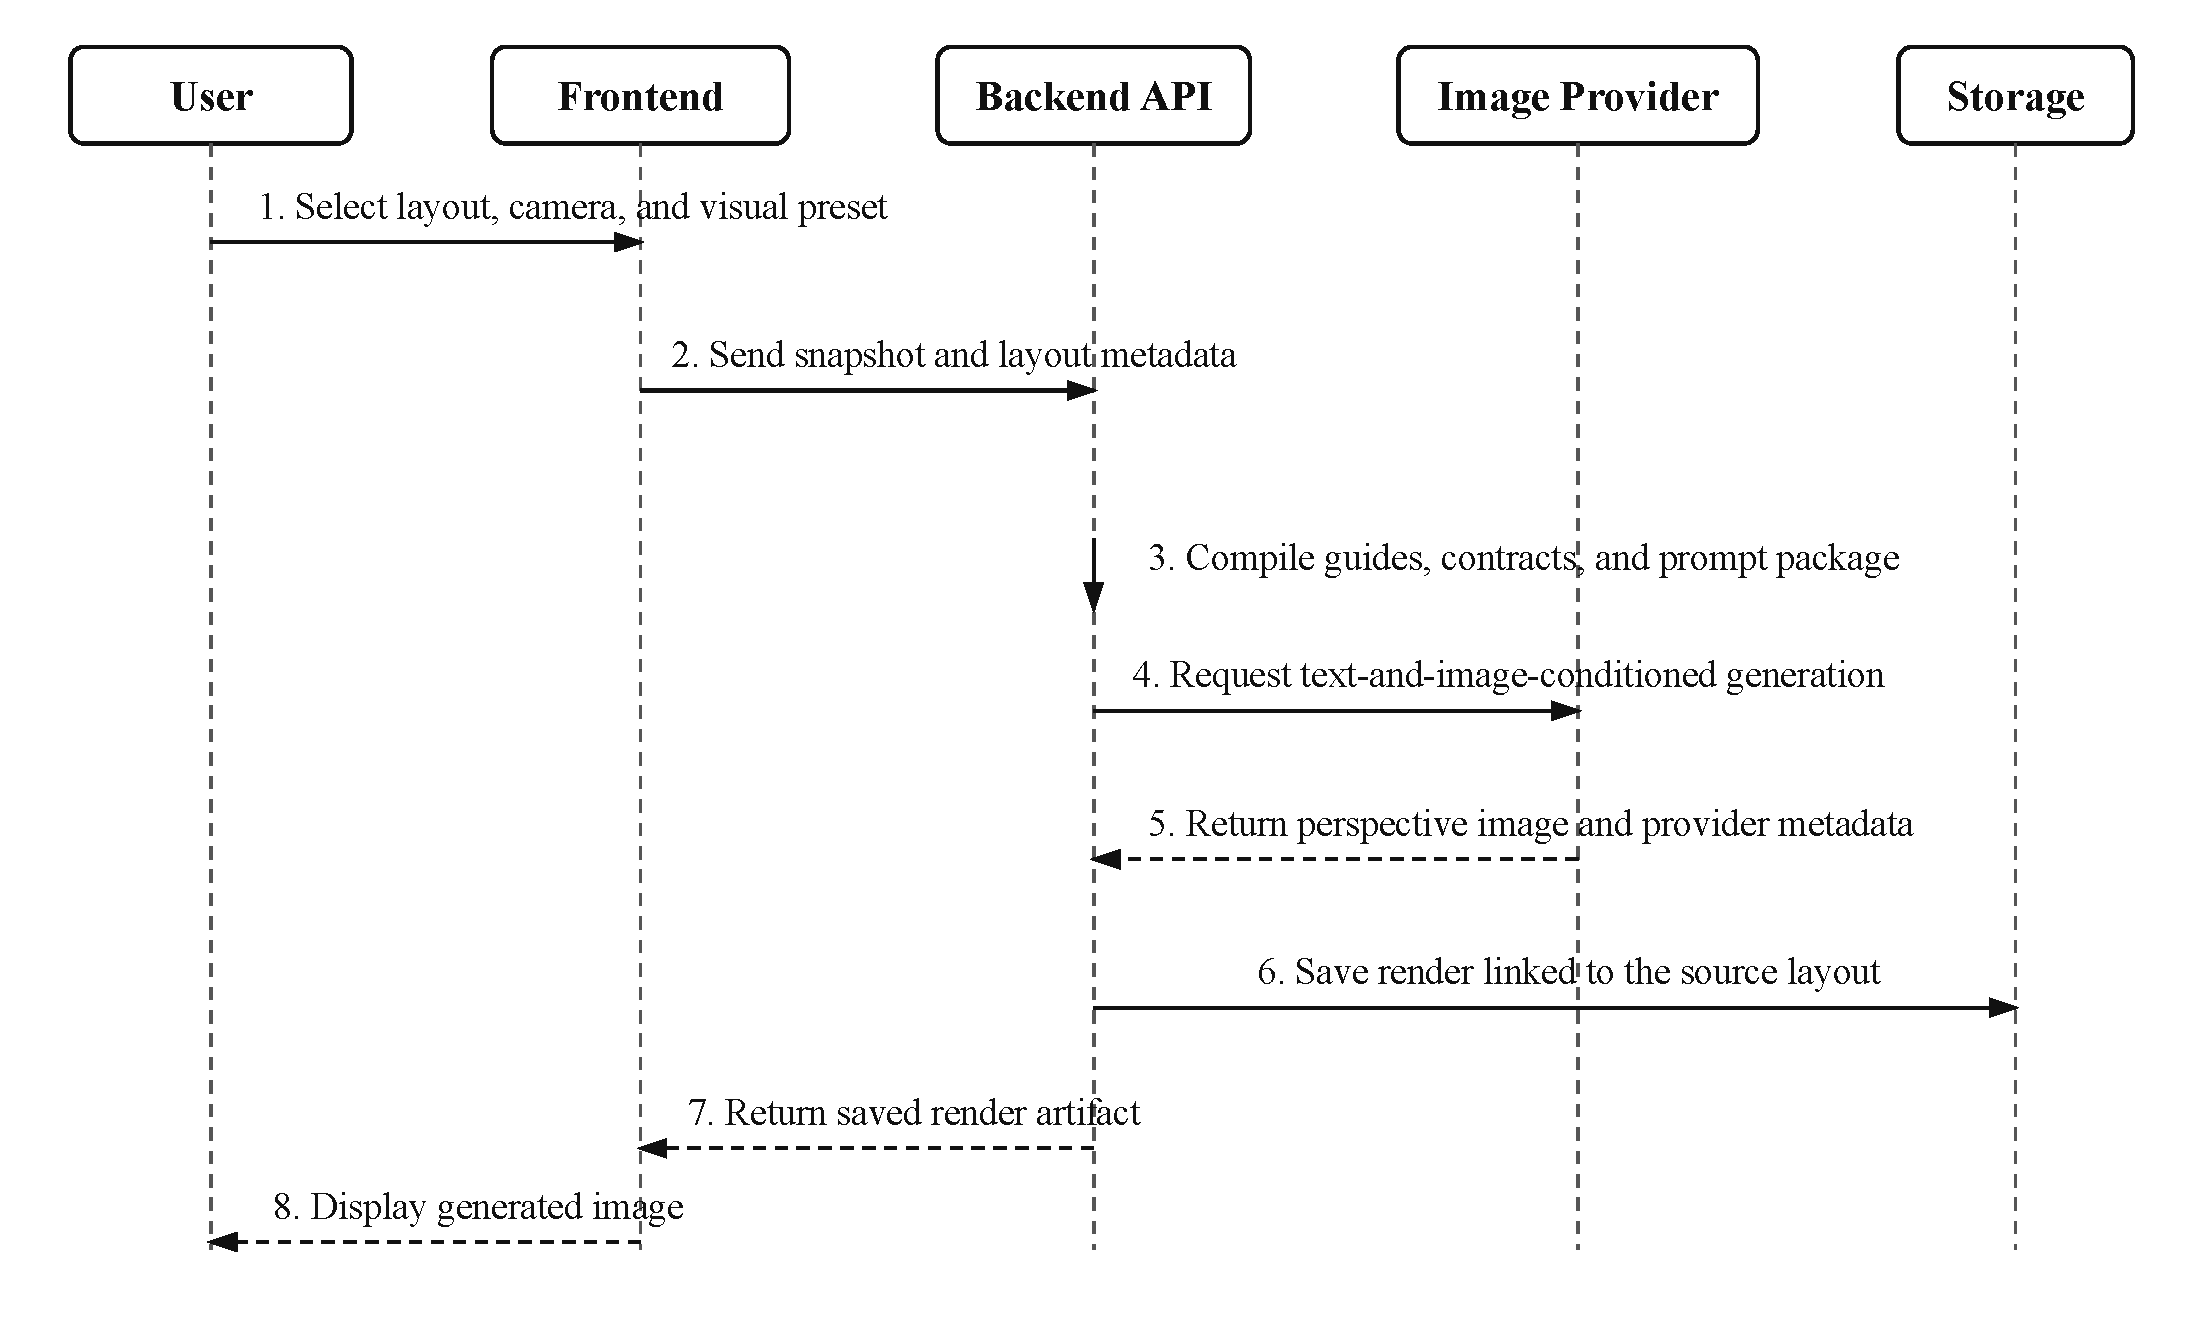
\includegraphics[width=\textwidth]{figures/chapter4/figure_04.pdf}
\caption{Sequence diagram of image generation from a 3D snapshot.}
\label{fig:6-4}
\end{figure}

The image-generation sequence in Figure~\ref{fig:6-4} keeps the 3D snapshot as the source of truth. Prompt compilation, provider call metadata, runtime, token usage, and saved render records are all tied back to the selected layout option.

Image generation and editing are also long-running operations. The backend reports progress before and after snapshot validation, prompt compilation, provider execution, and artifact persistence. Timeout, provider error, or invalid target-scope failures are returned as explicit status records so the user can retry, adjust the camera, or refine the target region without losing the selected layout.

\subsection{Database Design}\label{subsec:database-design}

The database schema separates shared assets, user data, and generated content. Asset and asset-file tables store inventory information and model files. User and auth-session tables handle login state. Saved layout cases group related layout variants, while saved layouts store floorplan JSON, design JSON, styled result JSON, and option metadata. Generated renders store prompt, model name, image bytes or storage path, source layout id, case id, option id, and render metadata.

This separation allows the system to reuse the same inventory across users while keeping saved designs and generated images user-specific. It also supports later auditing because a render can be traced back to the layout, case, option, prompt, and model configuration that produced it.

Figure~\ref{fig:6-5} presents the simplified database E-R diagram for these runtime entities.

\begin{figure}[!htbp]
\centering
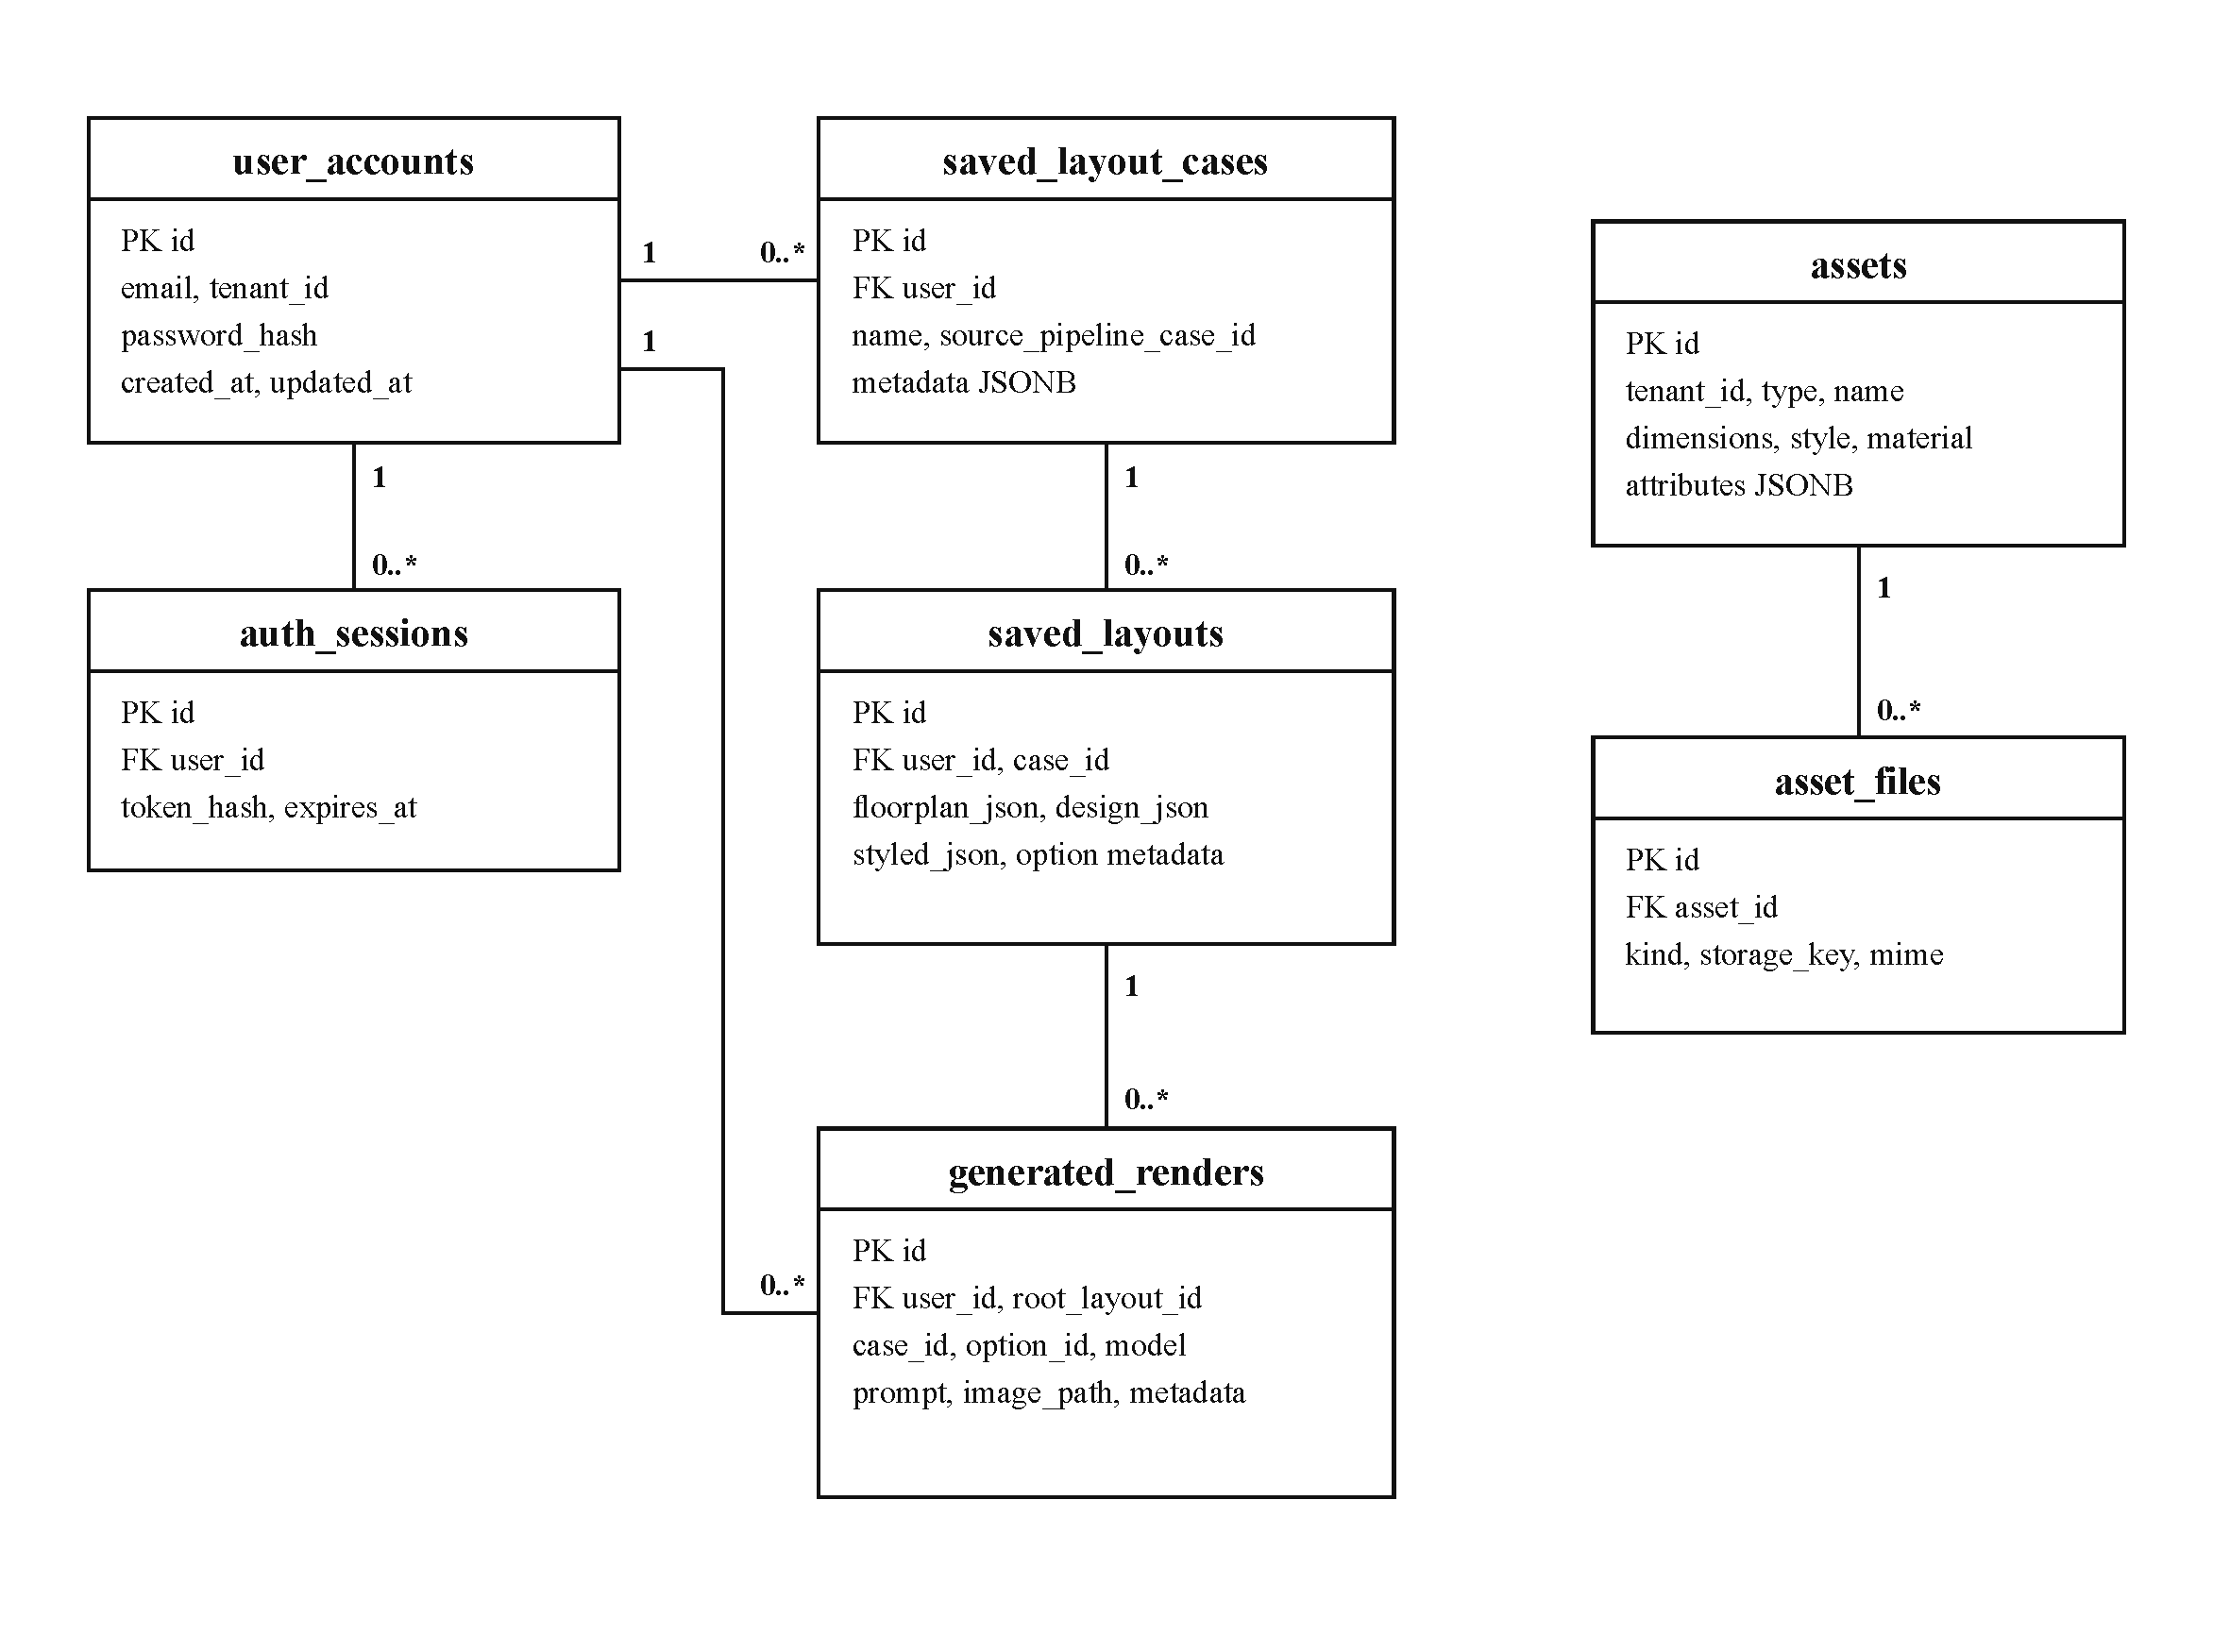
\includegraphics[width=\textwidth]{figures/chapter4/figure_05.pdf}
\caption{Simplified database E-R diagram showing the implemented entities and their main relationships. Detailed fields are listed in \hyperref[tab:6-1]{Table~6.1}.}
\label{fig:6-5}
\end{figure}

The relational schema in Figure~\ref{fig:6-5} keeps stable ownership and traceability fields in columns, while flexible layout and render payloads are stored as JSONB. This is suitable for a prototype whose layout schema evolves during experiments but still needs account-level isolation and reproducible links between layouts and renders.


\begingroup
\footnotesize
\setlength{\tabcolsep}{3pt}
\renewcommand{\arraystretch}{1.05}
\begin{xltabular}{\textwidth}{|>{\raggedright\arraybackslash}X|>{\raggedright\arraybackslash}X|>{\raggedright\arraybackslash}X|>{\raggedright\arraybackslash}X|}
\caption{Summary of the main database entities.}\label{tab:6-1}\\
\hline
Entity/table & Key fields & Main relationship & Role in the system \\
\hline
user\_accounts & id, email, tenant\_id, password\_hash & Owns sessions, layouts, renders & Authenticated identity and tenant boundary. \\
\hline
auth\_sessions & id, user\_id, token\_hash, expires\_at & Belongs to user & Login state without storing raw access tokens. \\
\hline
assets & id, tenant\_id, type/name, dimensions, attributes & Has asset\_files & Shared or tenant inventory metadata. \\
\hline
asset\_files & id, asset\_id, kind, storage\_key, mime & Belongs to asset & File references for models and images. \\
\hline
saved\_layout\_cases & id, user\_id, name, source\_\allowbreak pipeline\_\allowbreak case\_\allowbreak id & Has saved\_layouts & Groups layout options from one request. \\
\hline
saved\_layouts & id, user\_id, case\_id, floorplan\_json, design\_json, styled\_json & Belongs to case/user & Editable layout option payload. \\
\hline
generated\_renders & id, user\_id, root\_layout\_id, case\_id, option\_id, prompt, image\_path, meta & Belongs to layout/user & Generated or edited images and metadata. \\
\hline
design\_knowledge & id, tenant\_id, title/content, category/tags, source/meta & Shared or tenant-scoped & Reusable planning and prompting rules. \\
\hline
\end{xltabular}
\endgroup

\section{Application Building}\label{sec:application-building}

\subsection{Libraries and Tools}\label{subsec:libraries-and-tools}

The project uses a web stack and AI-service integration rather than a single monolithic desktop application, and Table~\ref{tab:6-2} summarizes the main tools and libraries used in the implemented system.


\begingroup
\small
\setlength{\tabcolsep}{4pt}
\renewcommand{\arraystretch}{1.15}
\begin{xltabular}{\textwidth}{|>{\raggedright\arraybackslash}X|>{\raggedright\arraybackslash}X|>{\raggedright\arraybackslash}X|}
\caption{Main libraries and tools used in the system.}\label{tab:6-2}\\
\hline
Purpose & Tool or library & Role in the project \\
\hline
Frontend application & React, TypeScript, Vite & Build the design workspace, account screens, and frontend state management. \\
\hline
2D editing & HTML Canvas and React components & Render and edit room geometry, openings, and furniture footprints. \\
\hline
3D preview & Three.js & Render the room shell, openings, furniture assets, proxy geometry, lighting, and camera views. \\
\hline
Backend API & FastAPI, Pydantic & Expose pipeline, auth, inventory, saved-layout, artifact, and image-rendering endpoints. \\
\hline
Persistence & PostgreSQL & Store inventory, users, sessions, saved layouts, and generated renders. \\
\hline
AI services & OpenAI-compatible text and image APIs; \texttt{gpt-5.4-mini} and \texttt{gpt-image-2} & Run LLM planning stages, visual preflight, and image generation/editing. \\
\hline
Geometry/evaluation & Shapely, Pillow, NumPy, image metrics & Score room geometry, overlaps, image structure, and visual outputs. \\
\hline
Deployment & Docker Compose and environment variables & Run the service and database with consistent local configuration. \\
\hline
\end{xltabular}
\endgroup

\subsection{Implemented Main Functions}\label{subsec:implemented-main-functions}

The implemented application covers three parts of the thesis workflow. First, the user-facing workspace supports room input, 2D editing, layout-variant review, 3D preview, image rendering, and saved artifacts.

Second, the backend pipeline records semantic intent, object quantities, solver outputs, style decisions, and final variants as separate artifacts instead of directly trusting LLM-generated coordinates. This makes each run inspectable for debugging and reproducible for benchmark evaluation.

Third, the experiment runners reuse these artifacts to evaluate layout generation in Chapter 7 and image generation and editing in Chapter 8. They remain separate from the interactive API path, while sharing the same core schemas and processing modules.

\hyperref[tab:6-3]{Table~6.3} summarizes the implementation scope and the main delivered artifacts. It intentionally describes functional implementation areas instead of exact source-size counts, because algorithmic quality is evaluated separately in Chapters 7 and 8.


\begingroup
\small
\setlength{\tabcolsep}{4pt}
\renewcommand{\arraystretch}{1.15}
\begin{xltabular}{\textwidth}{|>{\raggedright\arraybackslash}X|>{\raggedright\arraybackslash}X|>{\raggedright\arraybackslash}X|}
\caption{Implementation scope and main delivered artifacts.}\label{tab:6-3}\\
\hline
Item & Delivered artifact & Role in the system \\
\hline
Backend source & Backend API, application services, planning modules, solver integration, database adapters, and image-flow backend & Implements authentication, inventory access, layout generation, artifact retrieval, image rendering, saved layouts, and generated-render storage. \\
\hline
Frontend source & React workspace, 2D canvas editor, 3D preview, account UI, layout variant panel, and render controls & Provides the interactive user workspace for room editing, variant review, preview, rendering, and saved artifacts. \\
\hline
Evaluation scripts & Layout benchmark, ablation runners, robustness evaluation, image-flow evaluation, chart generation, and document figures & Supports the quantitative and qualitative evaluation reported in Chapters 7 and 8. \\
\hline
Main API groups & auth, account, inventory, pipeline & Four route groups cover login, persistence, inventory, and AI workflows. \\
\hline
Database entities & 7 core runtime tables & User/session data, inventory files, saved layouts/cases, and generated renders. \\
\hline
Preset assets & 13 styles, 13 lighting presets, 12 scenery presets & Reference options used by the image rendering workflow. \\
\hline
\end{xltabular}
\endgroup

The important delivered functions are the API groups, persistent entities, interactive editing workspace, layout-generation pipeline, 3D preview, image workflow, and evaluation runners.

The following figures illustrate the main implemented functions from the user perspective. \hyperref[fig:6-6]{Figure~6.6} shows the full workspace. Figures~\ref{fig:6-7}, \ref{fig:6-8}, and \ref{fig:6-9} enlarge the object library, room editor, 3D preview, and render controls so that the implemented controls remain readable on a portrait thesis page.

\begin{figure}[!htbp]
\centering
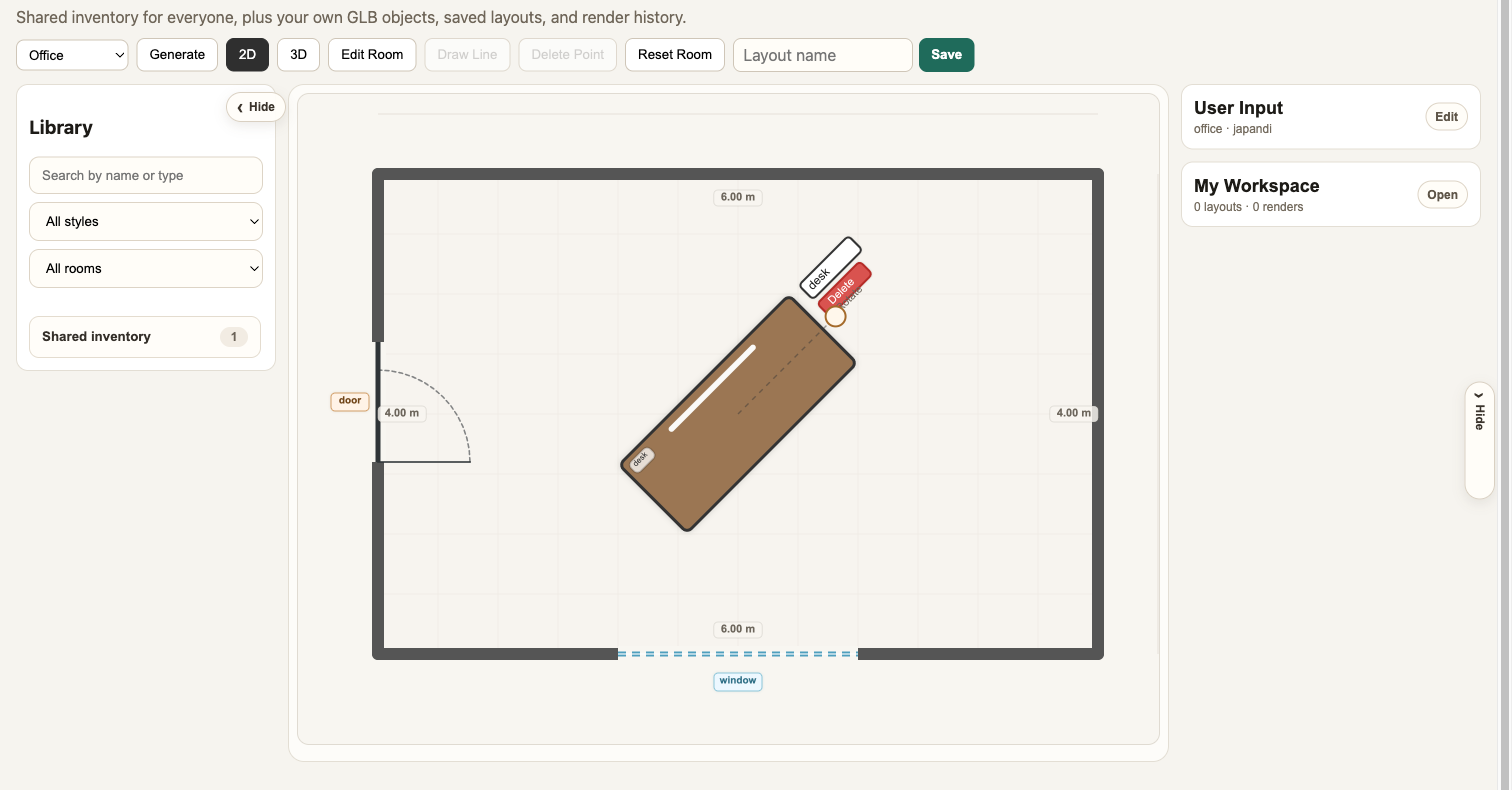
\includegraphics[width=0.92\textwidth]{figures/chapter4/figure_06.png}
\caption{Main implemented workspace. The left side contains the inventory and room-editing controls, the center contains the editable 2D floor plan, and the right side contains the design brief and generation controls.}
\label{fig:6-6}
\end{figure}

\begin{figure}[!htbp]
\centering
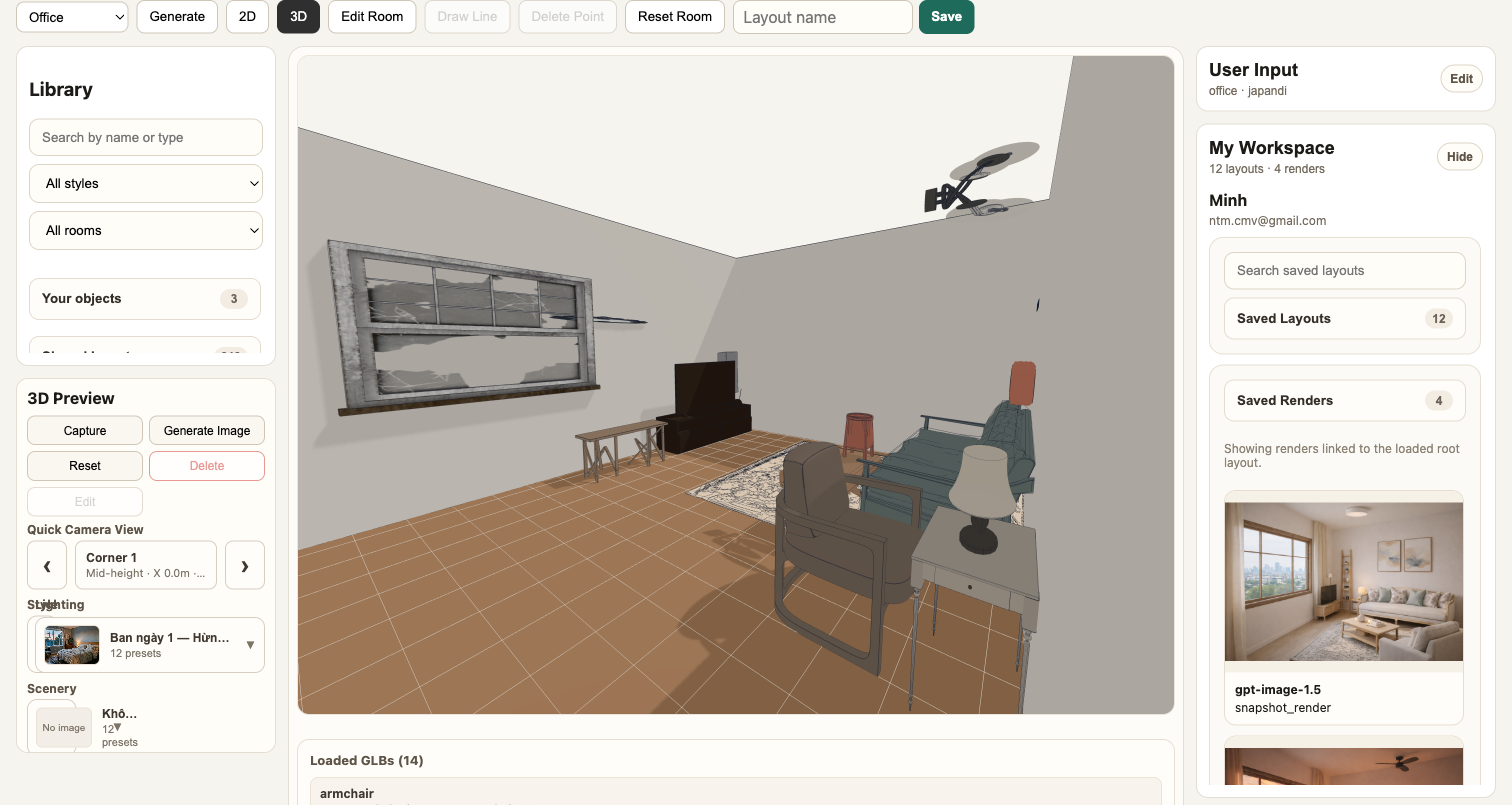
\includegraphics[width=0.92\textwidth]{figures/chapter4/figure_06_zoom.png}
\caption{Zoomed workspace panels showing the object library, camera and render controls, 3D preview viewport, and generated render panel.}
\label{fig:6-7}
\end{figure}

\begin{figure}[!htbp]
\centering
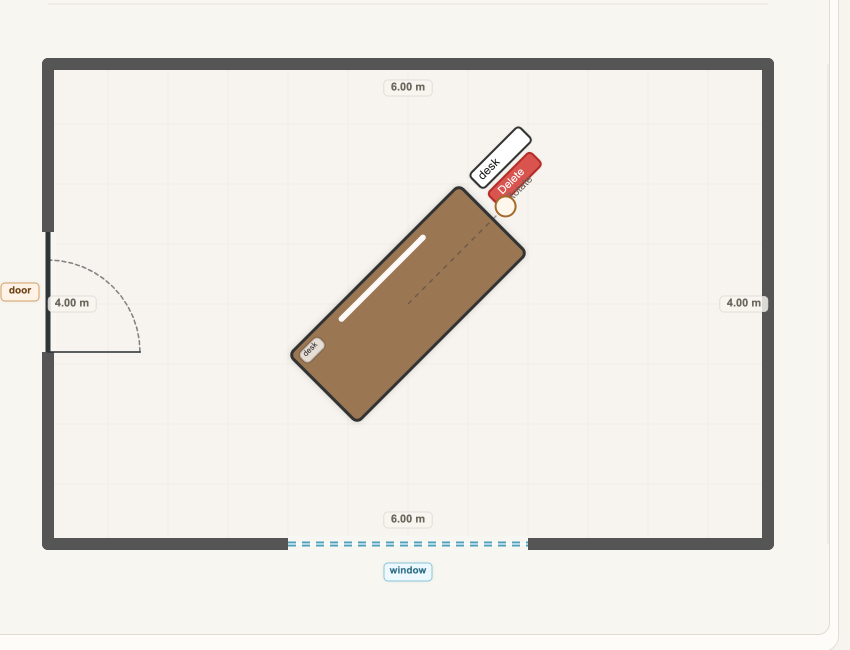
\includegraphics[width=0.92\textwidth]{figures/chapter4/figure_06_2d.png}
\caption{Cropped 2D room workspace showing the editable room boundary and fixed openings.}
\label{fig:6-8}
\end{figure}

\begin{figure}[!htbp]
\centering
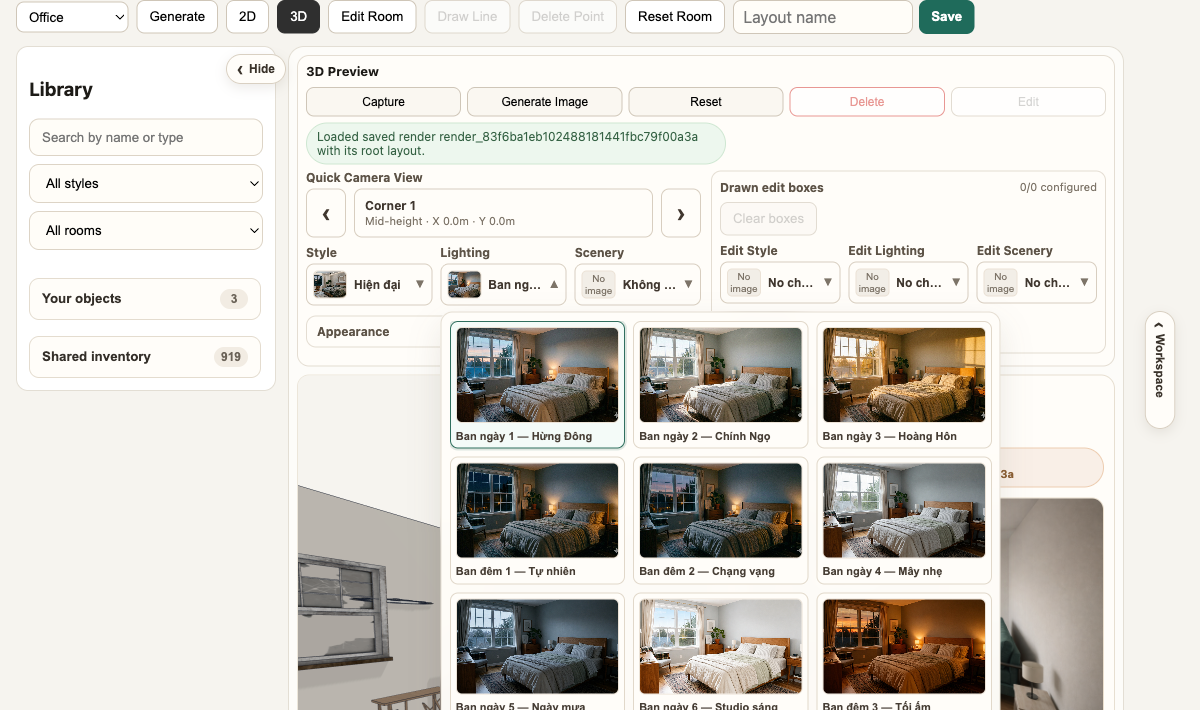
\includegraphics[width=0.92\textwidth]{figures/chapter4/figure_07.png}
\caption{3D preview and image-rendering controls.}
\label{fig:6-9}
\end{figure}

Figure~\ref{fig:6-10} shows the generated perspective render beside its 3D layout source, making the connection between the editable scene and the visualization output visible in the implemented interface.

\begin{center}
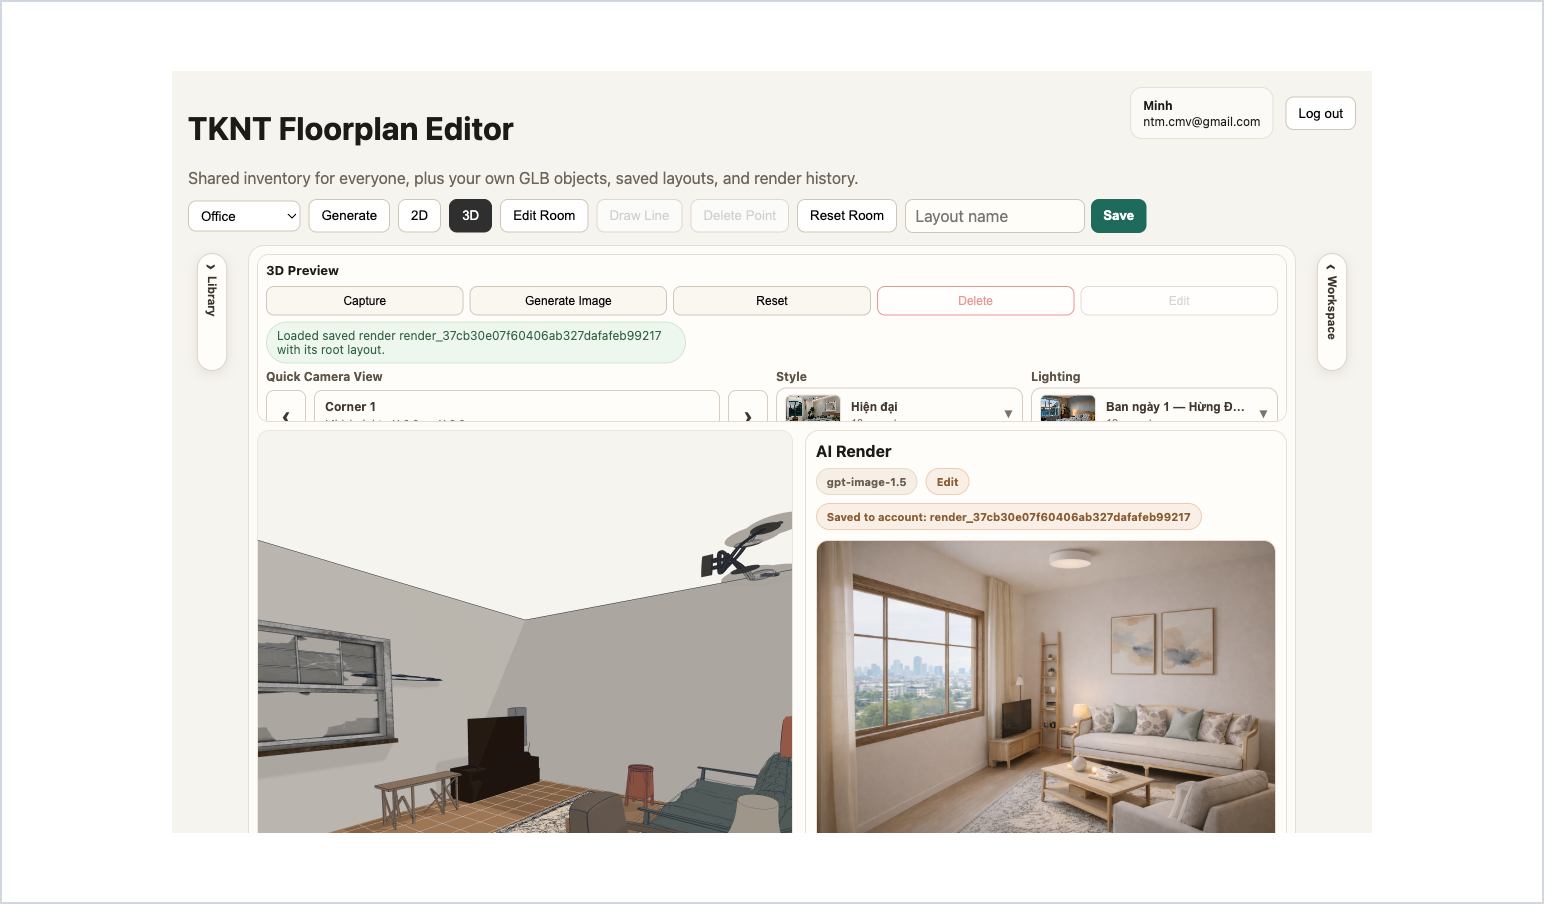
\includegraphics[width=0.84\textwidth]{figures/chapter4/figure_08.png}
\captionof{figure}{Generated render displayed beside the 3D layout source.}
\label{fig:6-10}
\end{center}


\section{Deployment}\label{sec:deployment}

The project includes configuration files for both local development and Docker-based execution. Docker Compose starts the backend service and PostgreSQL database with consistent environment variables. During development, the frontend can run separately with Vite and communicate with the backend through REST and server-sent event endpoints. Provider keys, database URLs, authentication secrets, and model settings are kept outside the source code through environment variables. This deployment is sufficient for thesis evaluation and local demonstration, while production deployment would require stronger monitoring, rate limiting, backup, and secret-management policies. Table~\ref{tab:6-4} summarizes the deployment components and the configuration responsibilities for each part.

\begingroup
\small
\setlength{\tabcolsep}{4pt}
\renewcommand{\arraystretch}{1.15}
\begin{xltabular}{\textwidth}{|>{\raggedright\arraybackslash}p{2.6cm}|>{\raggedright\arraybackslash}p{2.4cm}|>{\raggedright\arraybackslash}X|>{\raggedright\arraybackslash}X|}
\caption{Deployment components and configuration responsibilities.}\label{tab:6-4}\\
\hline
Component & Typical execution & Configuration & Security or storage note \\
\hline
Frontend & Vite development server or static build & Backend base URL, feature flags & Does not store provider keys. \\
\hline
Backend API & FastAPI service or Docker container & Database URL, auth secret, provider model settings, pipeline flags & Holds provider keys through environment variables; logs must not expose secrets. \\
\hline
PostgreSQL & Docker service or local database & Database name, user, password, port & Stores users, sessions, inventory, layouts, and render metadata. \\
\hline
Artifact storage & Local workspace folders in the prototype & Case directory, render directory, evaluation output paths & Stores reproducible pipeline artifacts, snapshots, generated images, and metrics. \\
\hline
AI providers & External API services & API keys, model names, retry and timeout settings & Calls are made only from backend-controlled code. \\
\hline
\end{xltabular}
\endgroup

For local execution, the frontend, backend, and database can be started separately during development. For Docker-based execution, Compose provides a repeatable backend and database setup. In both modes, secrets remain outside committed source files and are loaded at runtime through environment variables.
